\chapter{Strutture dati elementari}

\section{Che cos'è una struttura dati}
Gli insiemi rappresentano un concetto fondamentale per l'informatica e la matematica. Mentre gli insiemi matematici sono immutabili, gli insiemi manipolati dagli algoritmi possono crescere, ridursi o cambiare nel tempo. Per questo motivo questi insiemi sono detti \textit{\textbf{dinamici}}.

\dfn{Insieme Dinamico}{
    Sia n $\geq$ 0 e sia S = $\{e_1, e_2,..., e_n\}$  un \textit{\textbf{insieme}}, cioè una collezione di oggetti distinguibili, che si denotano come elementi (o attributi). Un insieme è detto \textit{\textbf{dinamico}} se e soltanto se la sua cardinalità può variare nel tempo, cioè può variare il numero dei suoi elementi.
}
 Gli algoritmi per la risoluzione di un problema possono richiedere vari tipi di operazioni da svolgere sugli insiemi.

\dfn{Struttura dati astratta}{
    Si dice \textbf{struttura dati astratta} un insieme dinamico definita da un punto di vista logico, descrivendo cioè soltanto le associazioni logiche tra i dati e le operazioni mediante le quali utilizzare la struttura.
}

Le \textbf{caratteristiche} principali che differenziano le strutture dati astratte sono:
\begin{itemize}
	\item La possibilità di cambiare o meno dimensione durante l'esecuzione (\textbf{dinamica} o \textbf{statica});
	\item Il fatto che i dati siano tutti dello stesso tipo oppure no (\textbf{omogenea} o \textbf{eterogenea});
	\item Il fatto che sia possibile accedere direttamente a un elemento, o che sia invece necessario scorrere tutti gli elementi precedenti (\textbf{accesso diretto} o \textbf{sequenziale});
\end{itemize}

\dfn{Struttura dati concreta}{
    Una struttura dati \textbf{concreta} è la rappresentazione nella memoria del computer di una struttura dati astratta.
}

\begin{example}
Un esempio di struttura dati astratta potrebbe essere una sequenza di numeri, una sua possibile struttura concreta può essere un vettore.
\end{example}

La caratteristica principale che differenzia le strutture di dati concrete è il fatto che i dati siano memorizzati in memoria in locazioni di memoria contigue oppure no. Le strutture dati vengono memorizzate in memoria ed esistono soltanto all'interno del programma che le utilizza; quando il programma termina, i dati inseriti nella struttura non sono più utilizzabili; non è possibile conservare dati in queste strutture, né usarle per comunicare dati tra un programma e un altro.

\subsection{Gli elementi di un insieme dinamico}
In una tipica implementazione di un insieme dinamico, ogni elemento è rappresentato da un oggetto i cui attributi possono essere esaminati e manipolati se c'è un puntatore all'oggetto. Per alcuni tipi di insiemi dinamici si suppone inoltre che uno degli attributi dell'oggetto sia una \textbf{chiave} di identificazione. Se le chiavi sono tutte diverse, possiamo pensare all'insieme dinamico come a un insieme di valori chiave. L'oggetto può contenere \textbf{dati satelliti}, che vengono trasportati in altri attributi dell'oggetto oppure includere ulteriori attributi che possono essere manipolati dalle operazioni svolte sull'insieme; questi attributi possono contenere dati o puntatori ad altri oggetti dell'insieme.

\subsection{Operazioni sulle strutture dati}
Le operazioni su un insieme dinamico possono essere raggruppate in due categorie: le \textbf{interrogazioni} che restituiscono semplicemente informazioni sull'insieme; le \textbf{operazioni di modifica} che cambiano l'insieme.

Consideriamo un insieme con una relazione d'ordine $\leq$ e assumiamo che l'elemento \textsc{NIL} non sia mai presente all'insieme $(S, \leq)$. Per tale insieme possiamo definire le seguenti operazioni:

\begin{itemize}
	\item \textsc{Ricerca}(S,k): restituisce un elemento di S oppure \textsc{nil} se $k \notin S$.
	\item \textsc{Inserimento}(S,k): restituisce un nuovo insieme $S' = S \cup \{k\}$.
	\item \textsc{Cancellazione}(S,k): restituisce un nuovo insieme $S' = S \setminus \{k\}$.
\end{itemize}

Gli algoritmi per le operazioni sugli insiemi sfruttano le caratteristiche della rappresentazione dell’insieme e questo significa che le operazioni di modifica (inserimento e cancellazione) \textbf{dovranno mantenere intatte quelle caratteristiche} (ad esempio se devo aggiungere un elemento in una sequenza ordinata, devo aggiungerlo nella giusta posizione in modo da lasciare ordinata la sequenza). Chiaramente la ricerca è un operazione che non modifica la struttura dati e quindi preserva naturalmente le proprietà della struttura, mentre per le altre due, più vincoli avremo e più complesso sarà definire delle operazioni.

L'operazione di ricerca non si limita solo alla ricerca dell'elemento $k$ nell'insieme $S$, posso infatti ampliare tale operazione con altre operazioni di ricerca:
\begin{itemize}
	\item \textsc{Successore}(S,k): restituisce l'elemento con la più piccola chiave $a > k$.
	\item \textsc{Predecessore}(S,k): restituisce l'elemento con la più grande chiave $a < k$.
	\item \textsc{Minimo}(S,k): restituisce un puntatore all'elemento di S con la chiave più piccola.
	\item \textsc{Massimo}(S,k): restituisce un puntatore all'elemento di S con la chiave più grande.
\end{itemize}

\section{Array}
L'\textbf{array} è un potente strumento ampiamente usato in programmazione. Gli array servono ad immagazzinare ed organizzare i dati nella memoria di un calcolatore: la loro potenza deriva soprattutto dal fatto che forniscono un modo molto semplice ed efficace di eseguire e fare riferimento a computazioni su collezioni di dati che condividono attributi comuni.

\dfn{Array}{
    Un \textit{\textbf{array}} è un insieme \textit{\textbf{statico}}, in cui la \textit{dimensione} dello stesso è dunque \textit{prefissata}.
}

È possibile vedere gli array come un'applicazione fatta in questo modo:
\begin{equation}
\forall n \in \mathbb{N}, I_{n} = \{0,1,2,...,n-1\} \mapsto d \in A
\end{equation}
La quale ha come dominio l'insieme dei primi $n$ numeri e come codominio gli elementi contenuti nell'array. Per denotare quindi l'$i$-esimo elemento di $A$ si è soliti utilizzare la seguente notazione: $A[i] = d$.
Un modo alternativo per vedere l'array è considerarlo come l'unione di ciascuno dei suoi singoli elementi, ovvero:
\begin{equation}
A = \bigcup_{i=0}^{n-1} \{A[i]\}
\end{equation}

\subsection{Il problema dell'inserimento}
Affrontiamo ora il problema dell'inserimento in un array. Consideriamo quindi la nostra struttura dati fatta in questo modo:
\begin{center}
    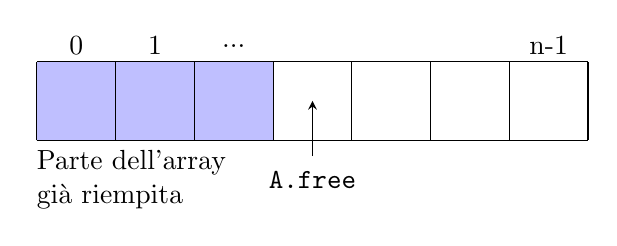
\begin{tikzpicture}
        \fill[blue, nearly transparent] (0,0) rectangle (3,-1);
        \draw (0,0) grid (7,-1);
        \node at (0.5,0.2) {0};
        \node at (1.5,0.2) {1};
        \node at (2.5,0.2) {...};
        \node at (6.5,0.2) {n-1};
        \node at (3.5,-1.5) {\texttt{A.free}};
        \draw [-stealth](3.5,-1.2) -- (3.5,-0.5);
        \node[align=left] at (1.2,-1.5) {Parte dell'array\\già riempita};
    \end{tikzpicture}
\end{center}

In questa struttura abbiamo un puntatore chiamato \texttt{A.free} che mira alla prima cella vuota dell'array. Se volessimo inserire un nuovo elemento, ammesso che l'array non sia pieno, si tratterebbe semplicemente di eseguire una operazione a \textit{tempo costante}. Questo perché l'array è una struttura che gode di \textbf{accesso diretto} alla memoria, grazie al fatto che le celle dell'array sono \textit{contigue}. Per i vari casi di studio che seguiranno, si faranno le seguenti assunzioni:

\begin{itemize}
    \item S è un insieme di dati dinamico contenuto in un intervallo contiguo di A (la cui lunghezza è predeterminata);
    \item S non ammette duplicati;
\end{itemize}

Per inserire un nuovo elemento all'interno del vettore, la prima operazione da effettuare è quella di assicurarsi che l'elemento non sia già presente nella struttura dati. Essendo l'array non ordinato, il problema della ricerca si riduce nell'esecuzione lineare di una lettura ed un confronto, a partire dall'inizio o dalla fine della struttura, fino all'esaurimento dell'array. Tale operazione ci tornerà parecchio utile sia per l'inserimento che per la cancellazione di un elemento in un vettore.

\begin{lstlisting}[label = lst:SearchInArray, language=asd, caption={Search(A,k)}]
pos = A.free - 1
while (A[pos] != k && pos >= 0) do
	pos = pos - 1
return pos
\end{lstlisting}

L'algoritmo \ref{lst:SearchInArray} restituisce la posizione dell'elemento nell'array se l'ha trovato, altrimenti restituisce -1. Andando a fare un'analisi approssimativa del codice è facilmente osservabile che l'algoritmo ha un \textit{tempo di esecuzione lineare} dato dal controllo sequenziale di ogni singola cella del vettore. Di conseguenza il caso peggiore, nel caso della ricerca di un elemento in un vettore non ordinato, è ottenuto nel caso in cui l'array sia pieno, ovvero quando \texttt{A.free = n-1}.

Grazie all'algoritmo di ricerca è possibile implementare gli algoritmi di inserimento e rimozione di un elemento. Infatti, prima di eseguire tali operazioni bisogna innanzitutto verificare la presenza dell'elemento nell'insieme. Nel caso dell'inserimento di un nuovo elemento, qualora il vettore dovesse essere già pieno, è possibile adoperare una funzione usiliaria \texttt{Resize} che effettui il ridimensionamento del vettore\footnote{Allocando una porzione di memoria maggiore ed eseguendo la copia degli elementi dell'array originale  nel nuovo vettore così ottenuto.}. Nel caso della cancellazione di un elemento, invece, non è necessario effettuare alcun ridimensionamento ma semplicemente sostituire all'interno della cella in cui si trova l'elemento da cancellare con il valore dell'ultimo elemento dell'array ed infine decrementare \texttt{A.free} di 1.

\begin{center}
	\begin{minipage}{0.4\textwidth}
	\begin{lstlisting}[label = lst:InsertInArray, language=asd, caption={Insert(A,k)}]
pos = Search(A, k)
if (pos == -1) then
	if (A.free == length(A)) then
		A = Resize(A)
	A[A.free] = k
	A.free = A.free + 1
\end{lstlisting}
\end{minipage}
\begin{minipage}{0.4\textwidth}
	\begin{lstlisting}[label = lst:DeleteInArray, language=asd, caption={Delete(A,k)}]
pos = Search(A, k)
if (pos >= 0) then
    A[pos] = A[A.free-1]
    A.free = A.free - 1
\end{lstlisting}
\end{minipage}

\end{center}

Consideriamo il caso in cui l'insieme dinamico memorizzato nell'array sia un insieme all'interno del quale è stata definita una relazione d'ordine $\leq$. In questa situazione ogni elemento dell'array deve soddisfare alla seguente condizione:
\begin{displaymath}
	\forall i \bigl(\ 1 \leq i \leq n \Rightarrow S[i]\leq S[i+1]\bigr)
\end{displaymath}
Grazie a questo vincolo aggiuntivo possiamo osservare che è possibile migliorare notevolmente le operazioni di ricerca. Infatti, nel caso dei vettori non ordinati, la ricerca dell'elemento massimo o minimo richiede sempre tempo lineare dovendo scorrere l'array nella sua interezza mentre, in un vettore ordinato, l'operazione richiede una singola operazione di lettura del primo elemento (nel caso della ricerca del minimo) o dell'ultimo elemento del vettore (nel caso della ricerca del massimo).

Nonostante i vantaggi ottenuti, nel caso della ricerca di un elemento, notiamo un peggioramento dal punto di vista computazionale nel caso delle operazioni di inserimento e cancellazione. Infatti, se volessimo inserire un nuovo elemento nell'array si può constatare facilmente che questo genere di operazione sia più complicata nel caso degli array ordinati in quanto prima di inserire un qualsiasi elemento sarà necessario cercare il suo precedente, far slittare gli elementi successivi e infine mettere l'elemento nella casella appena liberata.

Per un array non ordinato, al contrario, l'operazione si esegue facilmente a tempo costante in quanto basterebbe inserire il nuovo elemento alla fine del vettore. Scegliere i \textbf{vincoli della struttura dati} ha un impatto rilevante sulla complessità delle operazioni. Il punto di equilibrio dipenderà da fattori quali la dinamicità dell'insieme sul quale si sta operando, il numero di operazioni che si vogliono eseguire e la frequenza delle stesse. Da questo breve esempio si deduce che non esiste una struttura dati ``perfetta'': tutto dipende dalle operazioni che si vogliono eseguire su di esse.

\subsection{La ricerca binaria}
Come già detto in precedenza, mentre negli array non ordinati il problema della ricerca richiede sempre un tempo lineare, negli array ordinati il problema può essere risolto in \textit{tempo logaritmico}. Sfruttando infatti la proprietà dell'ordinamento è possibile definire un algoritmo ricorsivo chiamato \textsc{Ricerca-Binaria} oppure \textsc{Ricerca-Dicotomica} il quale confronta la chiave $key$ ricercata con quella dell'elemento centrale dell'array: se questa è uguale, la ricerca termina con successo, se è maggiore, la ricerca procede richiamando lo stesso metodo sulla prima metà dell'array mentre, se è minore, nella seconda metà dell'array. In sintesi \textsc{Ricerca-Binaria} opera nel seguente modo:
\begin{enumerate}
	\item Divide la sequenza che prende in ingresso determinando il valore $q= \lfloor n/2 \rfloor$;
	\item Effettua il controllo $S[q]=key$, dove $key$ è il valore da ricercare; se la condizione è falsa allora:
	\begin{enumerate}
		\item Se $S[q]<key$ allora richiama se stesso nella sottosequenza di destra;
		\item Se $S[q]>key$ allora richiama se stesso nella sottosequenza di sinistra.
	\end{enumerate}
\end{enumerate}

\begin{lstlisting}[label = lst:BinSearchRec, language=asd, caption={BinSearchRec(A,k,i,j)}]
if (i <= j) then
    q = @$\lfloor$@(i+j)/2@$\rfloor$@
    if (A[q] < k) then
        ret = BinSearchRec(A, k, q+1, j)
    else if (A[q] > k) then
        ret = BinSearchRec(A, k, i, q-1)
    else
        ret = q
else
    ret = -1
return ret
\end{lstlisting}

Ora andiamo a fare un'analisi di questo algoritmo per vedere se abbiamo effettivamente migliorato il tempo di esecuzione. Localmente ogni chiamata della funzione ha tempo costante $c$, quindi per calcolare il tempo di esecuzione dell'algoritmo basta fare \[T_{Bs}(n) = \sum_{l=0}^{h+1} c\] dove $l$ rappresenta il livello della chiamata che stiamo eseguendo ed $h+1$ è il livello che corrisponde o al caso $A[q] = k$ oppure al caso $i<j$ dove l'elemento non è presente. A questo punto bisogna capire chi è $h$. Per fare ciò ci basta osservare che ad ogni chiamata ricorsiva andiamo sempre a considerare la metà dell'array mentre nell'ultima chiamata si considera una sola cella. Quindi:

\begin{equation}
\frac{n}{2^h} = 1 \iff n = 2^h \iff \log_2(n) = \log_2(2^h) \iff \log_2(n) = h
\end{equation}

Sostituendo nella sommatoria, otteniamo:

\begin{equation}\label{eq:ricbin1}
    \sum_{l=0}^{h+1} c = \sum_{l=0}^{\log_2(n)+1} c = c \sum_{l=0}^{\log_2(n)+1} 1 = c\log_2(n) + c
\end{equation}

Dall'equazione \ref{eq:ricbin1} osserviamo che il tempo di esecuzione della ricerca binaria $T_{Bs}(n)$ è logaritmica rispetto alla dimensione dell'array il che rappresenta un notevole miglioramento rispetto all'algoritmo \textsc{Search(A,k)} il quale abbiamo visto avere un costo computazionale lineare rispetto alla grandezza del vettore. Tuttavia, nonostante il risparmio di tempo dato dalla ricerca binaria, non si può dire altrettanto per gli altri algoritmi di inserimento e cancellazione (\textsc{Insert} e \textsc{Delete}) i quali richiedono un tempo lineare rispetto alla dimensione del vettore. Infatti, inserire un singolo elemento all'interno di un vettore non ordinato prevede innanzitutto la ricerca della posizione corretta dove inserire l'elemento che ha un costo logaritmico, lo slittamento di una posizione degli elementi del vettore il quale può avere alla peggio un costo lineare se l'elemento viene inserito nella prima cella più il costo dato dall'assegnazione che viene eseguito a tempo costante:
\[T_{insert} = \log_{2}(n)+n+C\]

Invece, nel caso di un inserimento che necessita anche il ridimensionamento del vettore mediante la funzione \textsc{Resize} si ha un overhead lineare aggiuntivo dato dalla copia di tutti gli elementi.

Al fine di ridurre il tempo di esecuzione dato dall'operazione di ridimensionamento, si può pensare di allocare nuova memoria per una grandezza doppia rispetto alla lunghezza del vettore originale, anziché limitarsi ad aggiungere una sola cella. In questo modo infatti si riduce in maniera logaritmica la necessità di dover ridimensionare il vettore a fronte di un nuovo inserimento.

\section{Liste concatenate}

\dfn{Lista concatenata}{
    Una \textit{\textbf{lista concatenata}} è un insieme dinamico in cui ogni elemento ha una chiave (\textit{key}) ed un riferimento all'elemento successivo
    (\textit{next}) dell'insieme. È una struttura ad accesso \textit{\textbf{sequenziale}}. Il singolo elemento di una lista è chiamato \textit{\textbf{nodo}}.
}

Per capire meglio come poter definire una lista, proviamo a considerare la sommatoria dei primi $n$ numeri:

\begin{displaymath}
    \sum_{i=0}^{n} i = \left \lbrace \begin{array}{ll}
                            0 & \mbox{se } n = 0 \\
                            n + \displaystyle\sum_{i=0}^{n-1} & \mbox{se }n \geq 1
                        \end{array} \right.
\end{displaymath}

Con questa definizione possiamo calcolare la sommatoria dei primi $n$ numeri, la quale è pari a 0 se $n=0$ ed è pari a $n$ più la sommatoria dei primi $n-1$ numeri quando $n\geq 1$. Allo stesso modo, possiamo definire una lista $L$ nel seguente modo:
	\begin{equation}\label{definizione:listaconcatenata}
		L=\left\lbrace
		\begin{array}{lc}
			\varnothing & \mbox{se vuota}\\
			\mbox{Un nodo con un puntatore ad una lista L'} & \mbox{altrimenti}
		\end{array}
		\right.
	\end{equation}

Una lista può avere varie forme: può essere singolarmente o doppiamente concatenata, ordinata oppure no, circolare oppure no. In una lista \textbf{semplicemente concatenata} è presente, oltre all'attributo chiave, un secondo attributo chiamato \textit{\textbf{next}} contenente l'indirizzo di memoria del nodo successivo. Nelle \textbf{liste doppiamente concatenate} è presente anche l'attributo \textit{\textbf{prev}} contenente un puntatore al nodo precedente. Dato un nodo $x$, se $x.prev=NIL$, l'elemento $x$ non ha un predecessore e quindi è il primo elemento della lista, chiamato \textbf{testa} o \textbf{head} della lista. Se $x.next=NIL$, l'elemento $x$ non ha successore e quindi è l'ultimo elemento della lista, che è detto anche \textbf{coda} o \textbf{tail}. Un attributo $L.head$ punta al primo elemento della lista. Se $L.head=NIL$, la lista è vuota.

Se una lista è \textbf{ordinata} l'ordine lineare della lista corrisponde all'ordine lineare delle chiavi memorizzate negli elementi della lista; l'elemento minimo è la testa della lista e l'elemento massimo è la coda della lista. Una lista può essere \textbf{non ordinata}; gli elementi di questa lista possono presentarsi in qualsiasi ordine. In una \textbf{lista circolare}, il puntatore \textit{prev} della testa della lista punta alla coda e il puntatore \textit{next} della coda della lista punta alla testa.

Una struttura del genere ha i suoi vantaggi dal punto di vista computazionale, come l'inserimento e la cancellazione (se sono sull'elemento da cancellare) a tempo costante, ma anche i suoi svantaggi, ovvero proprio il fatto che si ha un accesso \textit{sequenziale} alla memoria. Ciò significa che, per raggiungere un elemento della lista, bisognerà necessariamente scorrere tutta la struttura fino al nodo richiesto.

\subsection{Ricerca in una lista concatenata}
Data la struttura particolare delle liste concatenate non è possibile accedere direttamente ad un qualsiasi elemento come accade negli array bensì è necessario scorrere ogni nodo a partire dalla testa fino a quando non si trova l'elemento desiderato. Questo significa che per accedere ad un nodo di una lista $L$ è necessario effettuare una semplice ricerca lineare che restituisce un puntatore al nodo ricercato. Anche supponendo di avere una lista ordinata doppiamente concatenata e voler implementare la ricerca binaria, per raggiungere l'elemento della sottosequenza di grandezza $n/2^{i}$ bisogna partire dall'indice mediano della sequenza precedente; quindi il costo complessivo sarà:
\begin{displaymath}
	\sum_{i=1}^{\log n} \bigl(\frac{n}{2^{i}}\bigl)=n\sum_{i=1}^{\log n} \bigl(\frac{1}{2}\bigl)^{i}=n-1
\end{displaymath}
\begin{center}
	\begin{minipage}{0.4\textwidth}
	\begin{lstlisting}[label = lst:SearchRec, language=asd, caption={SearchRec(L, k)}]
ris = NULL
if (L != NULL) then
    if (L->key = k) then
        ris = L
    else
        ris = Search(L->next, k)
return ris
\end{lstlisting}
\end{minipage}
\begin{minipage}{0.4\textwidth}
	\begin{lstlisting}[label = lst:SearchIter, language=asd, caption={SearchIter(L, k)}]
ris = NULL
tmp = L
while (tmp != NULL && ris = NULL) then
    if (L->key = k) then
        ris = tmp
    else
        tmp = tmp->next
return ris
\end{lstlisting}
\end{minipage}
\end{center}

\subsection{Inserimento in una lista non ordinata}

Dato un nodo $x$, l'algoritmo \textsc{List-Insert}(Algoritmo \ref{lst:InsertList}) inserisce un nodo con chiave \texttt{x} nella testa della lista concatenata sfruttando il fatto che ogni elemento della lista è indipendente dagli altri e non sono disposti in maniera contigua. Questa operazione prende il nome di \textbf{inserimento in testa}. Prima di eseguire l'inserimento bisogna invocare una funzione \textsc{NewNode} per la creazione di un nuovo nodo.
\begin{center}
\begin{minipage}{0.4\textwidth}
\begin{lstlisting}[label=lst:NewNode, language=asd, caption={NewNode(k)}]
tmp = AllocaNodo()
tmp->key = k
return tmp
\end{lstlisting}
\end{minipage}
\begin{minipage}{0.4\textwidth}
\begin{lstlisting}[label=lst:InsertList, language=asd, caption={Insert(L, k)}]
ret = Search(L, k)
if (ret == NULL) then
	tmp = NewNode(k)
	tmp->next = L
	L = tmp
return L
\end{lstlisting}
\end{minipage}
\end{center}
\subsection{Inserimento in una lista ordinata}
Inserire un nodo all'interno di una lista ordinata non ha lo stesso costo dell'inserimento in testa. Infatti prima di poter inserire il nodo bisogna garantire il vincolo dell'ordinamento andando a fare una ricerca della posizione esatta in cui andare ad inserire il nuovo nodo, più precisamente andando a cercare all'interno della lista il nodo \textbf{predecessore}. L'algoritmo che si ottiene avrà quindi un costo lineare dato dall'operazione di ricerca. Si ha così l'algoritmo \textsc{InsertInOrderedList(L,k)}.

\begin{lstlisting}[label=lst:InsertInOrderedList, language=asd, caption={InsertInOrderedList(L, k)}]
tmp = L
p = NULL
while (tmp != NIL && tmp->key < k) do	// Ricerca del predecessore
    p = tmp
    tmp = tmp->next
if (tmp == NIL || tmp->key > key) then // Inserimento di un nuovo nodo
    new = NewNode(tmp, k)
    if (p != NIL) then	// Se esiste il predecessore si aggiorna il successivo
        p->next = new
    else	// Altrimenti si inserisce in testa
        L = new
return L
\end{lstlisting}

\begin{lstlisting}[label = lst:InsertInOrderRec, language=asd, caption={InsertInOrder-Rec(L,k)}]
if (L == NIL || L->key > k) then
    L = NewNode(L, k)
else (if L->key < k) then
    L->next = InsertInOrderRec(L->next, k)
return L
\end{lstlisting}

\subsection{Cancellazione di un nodo in una lista}
La cancellazione di un nodo da una lista non può essere fatto con un costo minore del lineare, che sia ordinata o meno la lista. Infatti la cancellazione comprende due passi: la ricerca del nodo con la chiave $k$ e la cancellazione del nodo e l'aggiornamento dei puntatori del nodo precedente e di quello successivo. Si ottiene così l'algoritmo \textsc{Cancella}$(L,k)$. Si supponga che la lista non contenga duplicati.

\begin{center}
	\begin{minipage}{0.4\textwidth}
	\begin{lstlisting}[label=lst:DeleteIter,language=asd,caption={\textsc{DeleteIter}(L,k)}]
tmp = L
p = NULL
while (tmp != NULL && tmp->key != k) do
    p = tmp
    tmp = tmp->next
if (tmp != NULL) then
    if (p != NULL) then
        p->next = tmp->next
    else
        L = L->next
deallocate(tmp)
return L
\end{lstlisting}
\end{minipage}
\begin{minipage}{0.4\textwidth}
	\begin{lstlisting}[label=lst:DeleteRec, language=asd, caption={\textsc{DeleteRec}(L, k)}]
if (L != NULL) then
    if (L->key == k) then
        tmp = L
        L = L->next
        deallocate(tmp)
    else
        L->next = DeleteRec(L->next, k)
return L
\end{lstlisting}
\end{minipage}
\end{center}

\section{Stack e Code}
Gli stack e le code sono un primo esempio di struttura dati astratta che possono essere implementate sia con un array che con una lista concatenata.
\subsection{Stack}
\dfn{Stack}{
    Uno \textit{\textbf{stack}} è struttura dati avente politica di inserimento e cancellazione di tipo \textbf{LIFO}: Last In, First Out.
}
In una struttura di tipo stack gli inserimenti e le cancellazioni avvengono sempre e solo in testa alla lista ed è per questo motivo che il l'ultimo elemento ad essere stato inserito sarà sempre il primo ad essere estratto. Alcune operazioni in uno stack S sono:
\begin{itemize}
    \item \textsc{Push}(S, k), aggiunge l'elemento $k$ \textbf{in cima} alla lista;
    \item \textsc{Pop}(S), rimuove il primo elemento \textbf{dalla cima} della lista.
\end{itemize}

Sono possibili altre funzioni, come \textsc{VisualizzaInTesta}, \textsc{StackVuoto} o \textsc{StackPieno}, che rispettivamente mostrano qual è l'elemento in testa, controlla se lo stack è vuoto oppure se è pieno.
\subsection{Code}
\dfn{Coda}{
    Una \textit{\textbf{coda}} è una struttura dati avente politica di accesso e rimozione di tipo \textbf{FIFO}: First In, First Out.
}

Al contrario di uno stack, quindi, in una coda gli inserimenti avvengono in coda alla lista, mentre le cancellazioni avvengono in testa alla lista. Alcune operazioni possibili\footnote{Anche per le code è possibile definire altre funzioni come per gli stack.}in una coda Q sono:
\begin{itemize}
    \item \textsc{Queue}(S, k), aggiunge l'elemento $k$ in coda;
    \item \textsc{Dequeue}(S), estrae l'elemento in testa.
\end{itemize}

\begin{center}
\begin{minipage}{.45\textwidth}
	\centering
		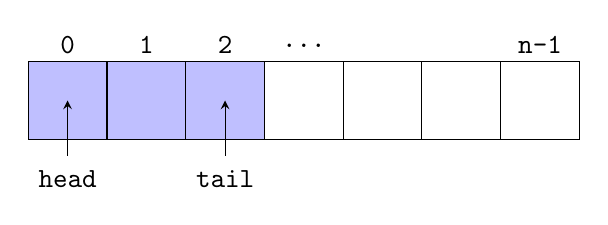
\begin{tikzpicture}
			[font=\ttfamily]
			\fill[blue, nearly transparent] (0,0) rectangle (3,-1);
			\draw (0,0) grid (7,-1);
			\node at (0.5,0.2) {0};
			\node at (1.5,0.2) {1};
			\node at (2.5,0.2) {2};
			\node at (3.5,0.2) {...};
			\node at (6.5,0.2) {n-1};
			\node at (2.5,-1.5) {tail};
			\node at (0.5,-1.5) {head};
			\draw [-stealth](0.5,-1.2) -- (0.5,-0.5);
			\draw [-stealth](2.5,-1.2) -- (2.5,-0.5);
		\end{tikzpicture}
	\captionof{figure}{Implementazione di una coda mediante array}
\end{minipage}\\
\begin{minipage}{.65\textwidth}
\centering
  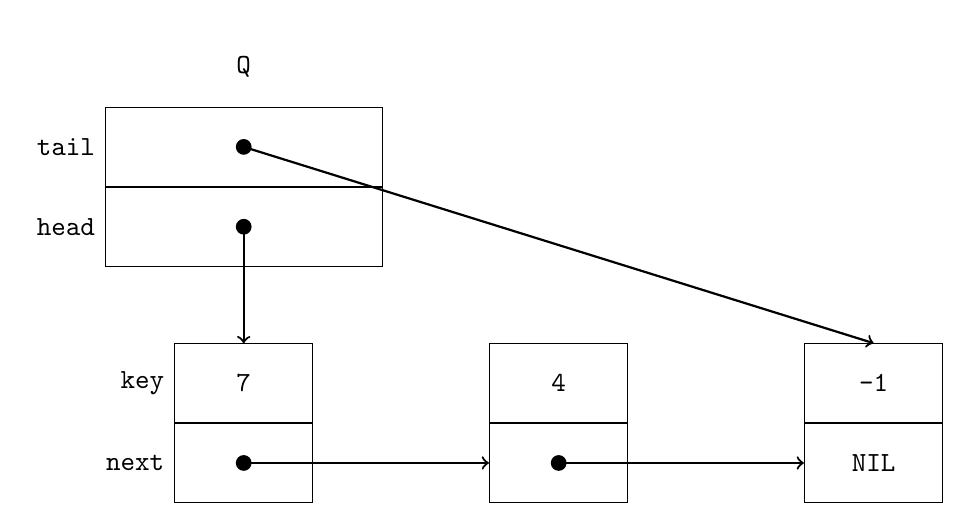
\begin{tikzpicture}[font=\ttfamily,minimum height=1cm,pointer/.style={fill, circle, minimum size=2mm, inner sep=0pt}]
	\node (tail) [rectangle,draw,minimum width=10em] {};
	\node (head) [rectangle,draw,anchor=north,minimum width=10em] at (tail.south) {};
	\node [anchor=south] at (tail.north) {Q};
	\node [anchor=east] at (tail.west) {tail};
	\node [anchor=east] at (head.west) {head};

	\node (a)[rectangle,draw,minimum width=5em] at (0,-3){7};
	\node (b)[rectangle,draw,anchor=north,minimum width=5em] at(a.south){};
	\node [anchor=east] at (a.west) {key};
	\node [anchor=east] at (b.west) {next};

	\node (c)[rectangle,draw,minimum width=5em] at (4,-3){4};
	\node (d)[rectangle,draw,anchor=north,minimum width=5em] at(c.south){};

	\node (e)[rectangle,draw,minimum width=5em] at (8,-3){-1};
	\node (f)[rectangle,draw,anchor=north,minimum width=5em] at(e.south){NIL};

	\draw[->,thick](tail.center) coordinate[pointer] -- (e.north);
	\draw[->,thick](head.center) coordinate[pointer] -- (a.north);
	\draw[->,thick](b.center) coordinate[pointer] -- (d.west);
	\draw[->,thick](d.center) coordinate[pointer] -- (f.west);
\end{tikzpicture}
\captionof{figure}{Implementazione di una coda mediante liste concatenate}
\end{minipage}
\end{center}
